\subsection{Questão de Pesquisa 4}

\textbf{Qual o foco da contribuição de pesquisa realizada em SOC e relacionada com qualidade de serviço? }
\\[0.01in]

Com o intuito de responder a esta questão, foi feita uma avalia\c c\~{a}o da distribui\c c\~{a}o dos 
artigos em rela\c c\~{a}o ao tipo de pesquisa (conforme discutido na Se\c c\~{a}o~\ref{sec:review_method}). 
O \emph{bubble plot} na Figura~\ref{fig:bubbleplot-QoSRes}  apresenta tal distibui\c c\~{a}o, novamente sendo importante ressaltar que o n\'{u}mero total de artigos nos gr\'{a}ficos \'{e} superior ao n\'{u}mero total de artigos analisados--- uma vez que alguns artigos apresentam contribui\c c\~{o}es tanto em termos de uma nova solu\c c\~{a}o proposta quanto em termos de avalia\c c\~{a}o e/ou valida\c c\~{a}o. Por exemplo, Huang et al. prop\~{o}e um modelo estoc\'{a}stico para representar e raciocinar sobre dependabilidade em um ambiente de SOC, ao mesmo tempo que valida formalmente tal proposta por meio de provas de teoremas~\cite{huang:scc2011}.

\begin{figure*}[htb]
\centering
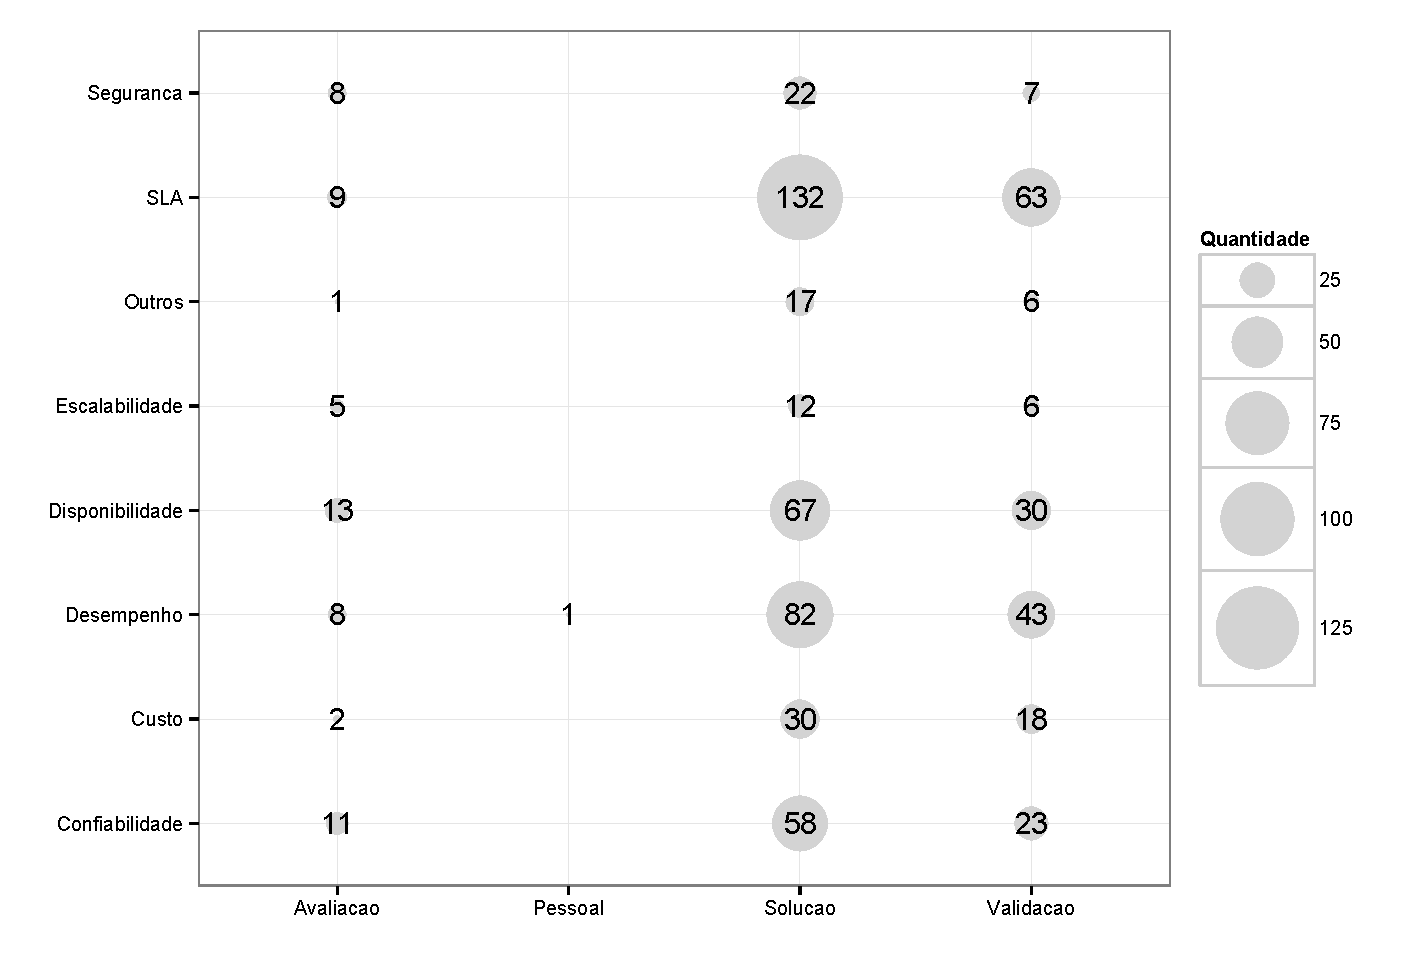
\includegraphics[scale=0.55]{imagens/pesquisaContexto2.pdf}
\caption{\emph{Bubble plot} com a distribui\c{c}\~{a}o envolvendo Tipo de Pesquisa e Contexto}
\label{fig:bubbleplot-QoSRes}
\end{figure*}

Esta investiga\c c\~{a}o revelou que 99 artigos ou 40.7\% do total apresentam, al\'{e}m de uma nova solu\c c\~{a}o relacionada \`{a} qualidade de servi\c cos em SOC, uma validação da proposta por meio de experimentos e simulações empíricas (e.g.  ~\cite{jeong:fqs2009,ardagna:jss2010,huang:scc2011,binshtok:icsoc2009}). Por outro lado, 141 artigos s\~{a}o propostas de solu\c c\~{o}es que não apresentam validações empíricas, isto é, carecem de experimentos que demonstrem a viabilidade e benefícios da(s) técnica(s) propostas. Entre esses artigos podemos citar \cite{filieri:faa2012,nascimento:splc2011,balfagih:icime2011,Clark:2009}. Finalmente, 22 artigos (9\%) foram classificados como avaliação, sendo que 15 apresentam, al\'{e}m de uma nova solu\c c\~{a}o relacionada \`{a} qualidade de servi\c cos em SOC, uma avaliação de técnicas correlatas em casos de uso reais, avaliando as limitações e benefícios das soluções existentes, e 7 artigos (2\%) somente avaliam em casos de uso reais propostas existentes identificando seus benefícios e limitações.

Esses n\'{u}meros revelam que a \'{a}rea de pesquisa de qualidade de servi\c co em SOC ainda est\'{a} em uma fase de amadurecimento naquilo que se refere ao uso e adoção em casos de uso reais das propostas, dada o baixo percentual dos artigos classificados como avaliação (9\%), o que indica a necessidade de mais pesquisas capazes de comparar diferentes técnicas já existentes. Também observou-se que um percentual significativo das contribui\c c\~{o}es simplesmente apresentam novas abordagens ou fazem compara\c c\~{o}es envolvendo a pr\'{o}pria t\'{e}cnica proposta (58\%) --- o que pode levar a conclus\~{o}es tendenciosas. 